\documentclass[paper-main.tex]{subfiles}

\begin{document}

In this section, we explore how this demonstration can be used to teach a selection of signal processing techniques. 
We use complex audio signals (such as music and speech) as a natural successor to the constant and wandering tones used in Sections~\ref{sec:single_tone} and~\ref{sec:viterbi_wandering} respectively.
As complex audio signals are not quasi-monochromatic, the Viterbi algorithm as used in Section~\ref{sec:viterbi_wandering} is not directly applicable here. 
Instead, we use a hierarchy of passive filters which suppress noise, yet do not assume any specific form of the signal, unlike the Fourier-based maximum likelihood filter which is tuned to the sinusoidal signals in Section~\ref{sec:single_tone} and Appendix~\ref{app:sinusoid_likelihood}.

We use the Michelson interferometer as an ``optical microphone'', where a laser is used to detect sound instead of the electrical components in a conventional microphone.
Optical microphones have precedence in the laser microphones~\cite{laser_microphone} which are (or were historically) used in the defense industry and operate on a variety of related principles. 
%We use the term ``optical microphone'' to distinguish this technology from those previous technologies.
Our objective is to play a recording of speech or music through the speaker attached to mirror M2 (see Fig.~\ref{fig:ifo_schematic_webcam}), record the resulting interference pattern, and then recover the original signal via a selection of signal processing techniques. 


This analysis is indirectly related to the advanced signal processing techniques required to extract gravitational-wave signals. 
Instead, the apparatus serves as an independent demonstration for a broader physics and engineering audience, particularly in undergraduate laboratories. 
We describe additional hardware components required for this demonstration in Section~\ref{sec:photodiode} and the initial results in Section~\ref{sec:initialResultsOpMic}. 
We consider a selection of filter techniques, details of which can be found in the Supplementary Material and we refer the reader to Refs.~\cite{Mitra:2011, Lyons:2011, Stein:2000, OpenheimSchaferBuck:1999, PrakisManolakis:1996,10.5555/151045} for further information on digital signal processing. 
In Section~\ref{sec:opticalMicResults} we present the two best-performing analyses from our Supplementary Material. 



\subsection{Hardware modifications for the optical microphone}
\label{sec:photodiode}
The human ear can hear frequencies in the range of $\sim 20\,{\rm Hz}$--$20\,{\rm kHz}$. 
Speech intelligibility (being able to understand speech) requires frequencies up to $3\,{\rm kHz}$ and music requires up to and beyond $8\,{\rm kHz}$~\cite{speech_intelligibility}. Therefore, the optical microphone requires a sample rate of at least $16\,{\rm kHz}$ to capture both speech and music (adjusting for the Nyquist frequency). 
This cannot be achieved with the webcam used in Sections~\ref{sec:single_tone} and ~\ref{sec:viterbi_wandering} as it has a sampling rate of $30\,{\rm Hz}$ and thus can only ``hear'' frequencies below $15\,{\rm Hz}$.
To overcome this issue, we use a photodiode\footnote{A photodiode is an electrical component that acts as a regular diode when no light is incident on it, blocking any current flow in the reverse direction. As the intensity of incident light rises, it becomes increasingly conductive in the reverse direction.} at the output of the interferometer to achieve a sampling rate of $16\,{\rm kHz}$.

We place an OSRAM BPW21 photodiode in reverse-bias over an LM358 op-amp which together make a photo-detector that produces a voltage that depends on the incident intensity. 
The photodiode records the interference pattern at roughly the same off-center position as the webcam in Sections~\ref{sec:single_tone} and~\ref{sec:viterbi_wandering}, again chosen arbitrarily.
% I think this is probably not needed as I believe the editor comment is referring to the cloth screen over the photodiode, which is addressed below. 
%The photodiode is mounted on a piece of cloth stretched over a plastic frame, with the electrical leads connected underneath the cloth.
%This cloth screen mount was the ``grill cloth'' from the front of a dismantled commercial speaker, re-purposed. 
The voltage signal from the photo-detector is captured by an MCP3008 $10$-bit analog-to-digital converter (ADC) connected to a Raspberry Pi Model 3 v1.2~\cite{RaspberryPi:online} (henceforth: Pi), which provides a convenient means to record the photodiode data.
Together, the circuit samples the signal at $\sim 16\,{\rm kHz}$. 
Resources for using the Pi and photodiode, including a circuit diagram, are described in Appendix~\ref{app:circuit_diagram}.

Sampling any frequency component of the analog signal above the Nyquist frequency of $8\,{\rm kHz}$ leads to aliasing\footnote{Folding of frequencies greater than half the sampling rate.} into the detected range. We include an anti-aliasing Sallen-Key filter~\cite{sallen_key_filter} tuned to $16\,{\rm kHz}$ before the ADC to prevent this from happening.
This component attenuates any frequencies above $8\,{\rm kHz}$, before they are digitally sampled. We also place a cloth screen over the face of the photodiode to reduce the incident intensity and avoid saturating the ADC -- an improvised, physical solution that could instead be replaced by scaling down the voltage electronically. This cloth screen was re-purposed grill cloth from a commercial speaker.
% It’s not clear what limited the sample rate to 16kHz, but it was likely non-optimal reading of the ADC by the Pi script.
% The ADC used (MCP3008) is quoted at 200kHz (or ksps, kilo samples per second).

%An updated schematic and a photograph of the entire optical microphone are shown in the left and right panels of Fig.~\ref{fig:ifo_schematic_podo}, respectively.
%See Appendix~\ref{app:circuit_diagram} for a diagram of the circuit. 

\subsection{Anti-aliased output}
\label{sec:initialResultsOpMic}

%The source audio was played through the speaker with the optical microphone recording for the full duration of the audio (around a minute long for most sources). 
We test the optical microphone with a variety of recordings, including the speech of different people and music ranging from simple melodies and rhythms to songs. 
During recordings, care is taken to minimize activity around the demonstration to reduce environmental noise coupling into the interferometer. 
The timeseries data is then directly converted to a .wav file and played as an audio recording using the \texttt{scipy.io.wavfile.write} function in Python~\cite{scipy,python}. 
When processing the results, we restrict our analysis to only the first $10\,{\rm s}$ of each observation (for efficiency), and only plot the first second here. 

The raw output of the optical microphone (with anti-aliasing) is noisy with a loud bass hum throughout. 
This can be explained by looking at the power spectral density (PSD) of the background noise (i.e., with the speaker switched off), as shown in Fig.~\ref{fig:psd_noise}. 
The spectrum is dominated by AC mains noise with power from the fundamental $50\,{\rm Hz}$ Australian mains power grid signal up to and beyond $8$th harmonic thereof. 
The mains signal is also present (but far weaker) in the background spectrum taken with the photodiode in darkness, suggesting that ambient lighting has a large contribution. 
Besides lighting, other possible contributions to the mains signal include air conditioning and the photodiode circuit itself. 
The appearance of harmonics of the mains noise is likely due to the non-linearity discussed in Appendix~\ref{app:intensity_derivation} (see also Ref.~\cite{feynman}). 
The spectrum in Fig.~\ref{fig:psd_noise} also has a broad feature at around $750\,{\rm Hz}$, the origin of which is yet to be determined.


Environmental noise reduction is an active area of research for gravitational-wave detectors~\cite{EfflerEtAl:2015}.
In some cases environmental noise sources can be removed or mitigated on site~\cite{CovasEtAl:2018}. 
Where this is not possible, noise subtraction can be done after data collection~\cite{DriggersEtAl:2019, DavisEtAl:2019}. 
One example is removal of spectral noise lines from the United States power grid operating at $60\,{\rm Hz}$~\cite{VajenteEtAl:2020}. 
 


\begin{figure}
	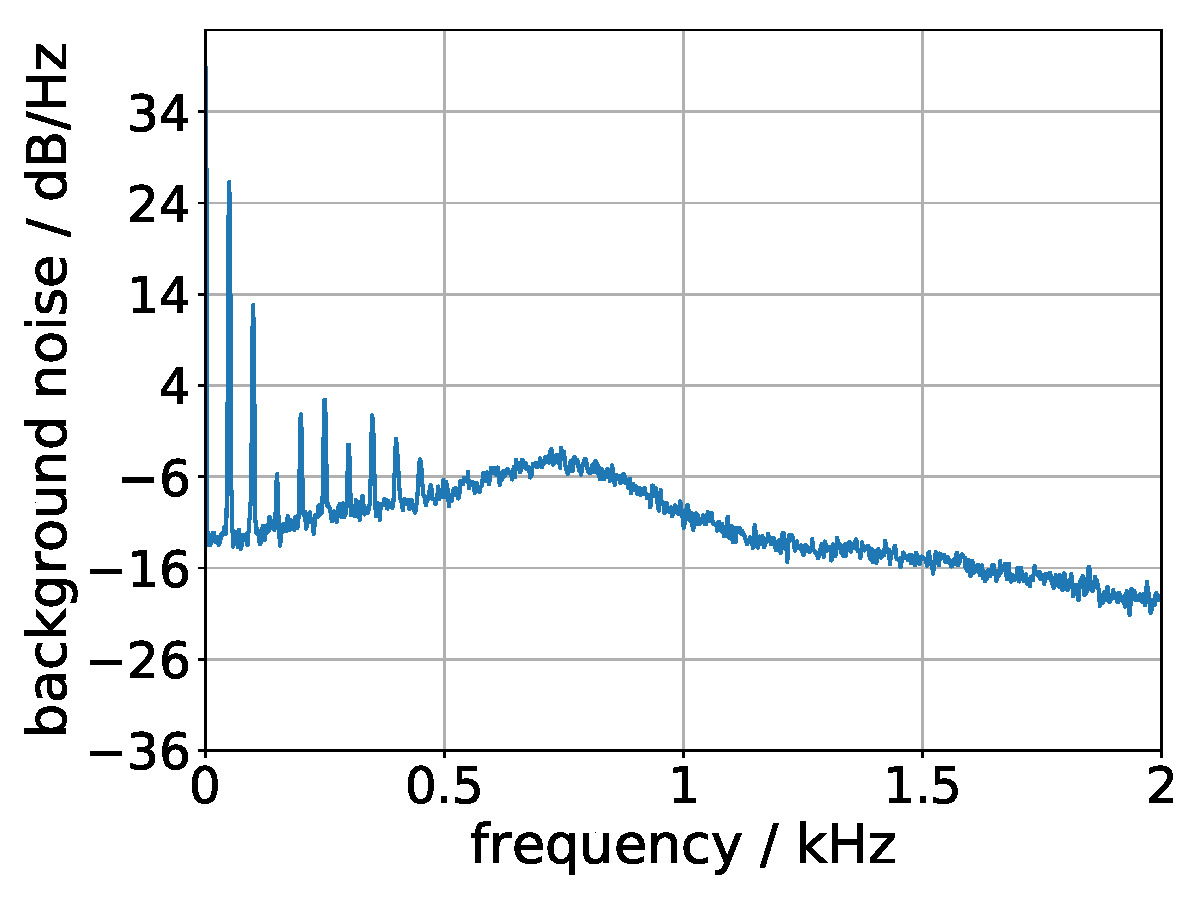
\includegraphics[width=.5\textwidth]{figures/psd_podo_14_6.pdf}
	\caption{\label{fig:psd_noise}
Power spectral density (PSD) of background noise from the optical microphone (with the speaker off). 
% Bottom: the PSD after applying a Butterworth bandpass filter (bottom panel) between the two frequencies marked with red, dashed lines. 
We see strong power from the $50\,{\rm Hz}$ mains hum and its harmonics (most likely from the photodiode circuit and the room’s lighting and cooling). Otherwise, the PSD is fairly white except for a peak at around 0.75~kHz. 
% After filtering we see strong attenuation (at least 3~dB) of all frequencies outside the band, but little change to the harmonics within the band.
}
\end{figure}


\subsection{Optical microphone results}
\label{sec:opticalMicResults}

\begin{figure*}
\begin{center}
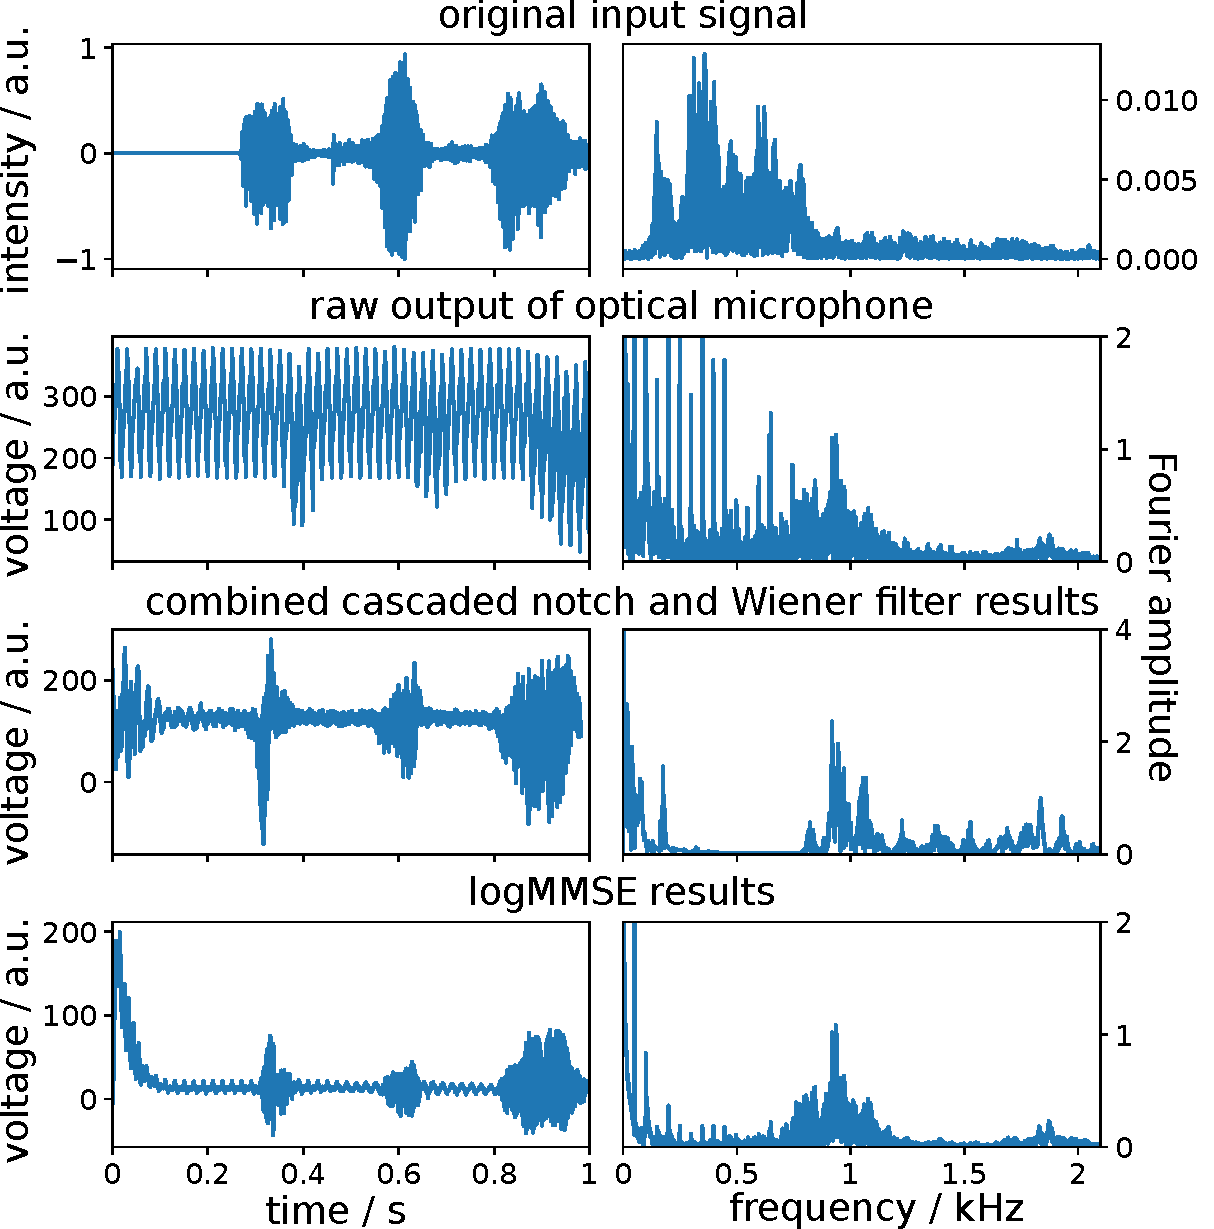
\includegraphics[width=0.95\textwidth]{figures/combined_highlight_results_melatos_labelled.pdf}
\caption{\label{fig:notchWienerLogMMSEResults}
Timeseries (left column) and frequency spectrum (right column) results with the optical microphone. 
The original input signal in the first row is a $1\,{\rm s}$ recording of an adult male voice (saying ``A cathode''). 
 The input signal is shifted by 0.12 s to the right to synchronize the manual delay from starting the recording with the Raspberry Pi and starting to play the source through the speaker. 
The second row shows the raw output from the optical microphone when the input from the first row is played. 
The third row shows the result of applying the notch and Wiener filter combined. 
The fourth row shows the result of applying the logMMSE estimator, where the rise at the start of the timeseries is an expected effect when filtering a signal of finite duration. 
}
\end{center}
\end{figure*}

We explore several filters to remove the $50\,{\rm Hz}$ mains hum and harmonics, and also to improve the speech intelligibility of the recording.
The accompanying Supplementary Material describes a range of analysis techniques that can be used as examples for the undergraduate laboratory. 
All filters are tested on the same $1\,{\rm s}$ long speech recording.
The results of this section are shown in Fig.~\ref{fig:notchWienerLogMMSEResults} which we refer to throughout. 
In Fig.~\ref{fig:notchWienerLogMMSEResults} the left and right columns show the timeseries and frequency spectrum respectively. 
The first row shows the input signal played through the speaker (see Fig.~\ref{fig:ifo_schematic_webcam}). 
The second row shows the raw output from the photodiode recording. 



In signal processing, the ideal filter would be one that:
(i) completely attenuates the undesired parts of the spectrum, 
(ii) does not change the rest of the spectrum, and 
(iii) smoothly transitions between these regions, as to not damage the time domain signal when seen under convolution. 
However, these three conditions cannot all hold at once. For example, if conditions (i) and (ii) hold, then the filter must be discontinuous at the boundary of the undesired region but this implies that the filter has ``infinite latency'' and so will affect (or damage) the time domain signal for infinite time~\cite{10.5555/151045}. Therefore, any filter must compromise between these three conditions. For speech intelligibility, this means that either: (i) some noise remains in the filtered recording, (ii) some of the speech content is lost as certain important frequencies are attenuated, or (iii) the speech is somewhat distorted in time. All three of these cases can, in extreme cases, worsen speech intelligibility beyond the unfiltered recording and so we choose filters that compromise between achieving the three conditions.
% https://en.wikipedia.org/wiki/Filter_(signal_processing)


In this section, we present results of two advanced signal processing analysis techniques applied to the optical microphone recordings. 
The techniques are only briefly described here and we refer the reader to the accompanying Supplementary Material for further details and some other analysis techniques. 


Firstly, we consider two signal processing techniques used in combination: the cascaded notch~\cite{10.5555/541204} and the Wiener filter~\cite{10.5555/151045}. 
A notch filter removes signals within a specific frequency range. 
We want to remove the $50\,{\rm Hz}$ mains noise and harmonics, therefore we use a cascaded notch filter where each notch is centered at each of the harmonics. 
The Wiener filter is an advanced statistical technique that makes use of statistical information from the speech data and noise. 
It amplifies parts of the signal with high signal-to-noise (SNR) ratio while suppressing parts with low SNR. 
The results of the combined cascaded notch and Wiener filter are shown in the third row of Fig.~\ref{fig:notchWienerLogMMSEResults} where the timeseries and spectrum are shown by the left and right panels respectively. 
Most of the mains noise is removed, however, the recovered voice sounds muffled and is not understandable. 


Secondly, we apply a speech enhancement technique. 
Ref.~\cite{SubjectiveComparison} compares $13$ speech enhancement methods, finding the log minimum mean-square-error (logMMSE) estimator to be the best, qualitatively, at recovering speech (see also Ref.~\cite{Ephraim1984SpeechEU_logMMSE} for details on the logMMSE estimator). 
We use an existing implementation of the logMMSE from~\cite{logmmse}.  
The logMMSE estimator results are shown in the bottom panel of Fig.~\ref{fig:notchWienerLogMMSEResults}. 
We see significant attenuation of the mains harmonics and general smoothing of the spectrum. 
Most of the background noise is removed, however, the logMMSE does not significantly enhance the speech as the voice sounds muffled and indistinct.
We find some improvement with music over speech. 
Simple chords and drums can be heard, however more composite sounds and complex melodies cannot be heard clearly. 
Our observations suggest that this is especially true for certain instruments, in particular flutes and violins sometimes can’t be heard at all. 
This could be a perceptual effect or a frequency dependence somewhere in the optical microphone.
Speculating, perhaps the speaker-mirror coupling is stronger at low frequencies and thus instruments like electric bass and drums are louder in the results.
To address these problems, we need to determine whether the signals that are audibly missing (the diction in the speech and complex melodies in music) are indeed being transmitted through the optical microphone at all. 
To determine this requires a better understanding of the system, as discussed in Section~\ref{sec:future_work}.



\end{document}
